\documentclass{article}

\usepackage{graphicx}
\usepackage{amsmath}
\usepackage{amssymb}
\begin{document}
\textbf{Siddharth Bhat (20161105)}

\section{Q1}
There is a component, call it A at site that initiated the transaction, and
components at each of the banks --- components B and C. Component B receives
the instruction from A. B checks that there is adequate money in the account, and
aborts if not.  Otherwise, B subtracts 10,000 from the account at B and
signals C to deposit 10,000 into the designated account at C. Component C
checks that the account exists, and aborts if not. Otherwise, C adds 10,000 to
the account and informs A of a successful conclusion. Once A has been
informed of the successful conclusion, it reports back to the user of
the success.

Due to the presence of time-outs, and since both $B$ and $C$ can send \texttt{Abort}
back to $A$, both crashes and failures such as insufficient funds are handled.
If $B$ or $C$ crash, the request times out; If there are insufficient funds,
then a \texttt{Abort} message is sent.
The coordinator sends a rollback message to all the participants.  Each
participant undoes their transactions using the undo log. Each participant sends an
acknowledgement to the coordinator.  The coordinator undoes the transaction
when all acknowledgements have been received.




\section{Q2}
\textbf{Consistency:} all nodes see the same data at the same time.
\textbf{Availability:} a guarantee that every request receives a response about whether it was successful or failed.
\textbf{Partition tolerance:} the system continues to operate despite arbitrary message loss.

The CAP theorem states that you cannot simultaneously have all three; you must make
tradeoffs among them. The CAP theorem is sometimes incorrectly described  as
the choice of picking consistency, availability, and partitioning during
\textbf{design time}. Really, the theorem allows for databases to choose
between these dynamically at \textbf{run time}.

When using NoSQL databases, we lose trade-off consistency for
a new property called \textbf{eventual consistency}.
This allows each system to make updates to data and learn of other updates
made by other systems within a short period of time, without being totally
consistent at all times. For most systems, knowing that it will reach
consistency in a short period of time is "good enough", when it allows
us to have consistency and availability as well!

\section{Q3}

\begin{itemize}
    \item Disk Block size $B = 4096 = 2^12 \text{bytes/block}$. Main memory is $M = 50 \text{MB} = 50 * 2^{20} \text{bytes}$. 
    \item Record $R$
        takes $R = 10^7\text{tuples} \times 10^2 \text{tuples/byte} = 10^9 \text{bytes}$.
    \item Disk IO is 15 msec.
    \item Number of blocks needed for relation: $R/B = \frac{10^9 \text{bytes}}{2^{12} \text{bytes/block}} = \frac{10^9}{2^{12}} \simeq 250,000 \text{blocks}$.
    \item Number of blocks in main memory: $M/B = \frac{50*2^{20}\text{bytes}}{2^{12} \text{bytes/block}} = 50 * 2^{8} = 12800 \text{blocks}$.
\end{itemize}

\subsubsection{Q3.1}
Since we are reading and storing in random order, we will need around $15\text{msec}$
for each block we are reading. 
We need to read and write each block of the relation $R$ once. This will take us
$15\text{msec} \times 250,000 \times 2= 7500 \text{seconds}$.

\subsubsection{Q3.2}
The original data may be stored on consecutive cylinders. Each of the 8192
cylinders of the Megatron 747 1 MB on average. We store the initial
data (which is $10^3$ MB) on 1000 cylinders, and we read 50 cylinders to fill
main memory (which is 50MB). Therefore we can read one cylinder with a single
seek time. We do not even have to wait for any particular block of the cylinder
to pass under the head, because the order of records read is not important at
this phase. It takes 6.4 seconds for the transfer of 12,800 blocks.
The writing part of phase 1 can also use adjacent cylinders to store the 20
sorted sublists. of records. They can be written out onto another 1000 cylinders.
Thus, the writing time for phase 1 is also about 2.15
minutes, or 4.3 minutes for all of phase 1.

On the other hand, storage by cylinders does not help with the second phase
of the sort. Thus, the second phase will still take about 125 minutes.

\subsubsection{Q3.3}

Replacing the disk by 4 disks


% Number of times we need to read into memory to read full relation: 
% $$\frac{\text{# of blocks needed for relation}}{\text{{# Number of blocks in main memory}} =\frac{10^9}{2^{12}} * \frac{1}{50 * 2^8} \simeq 20$$
% Each block needs both  a read and a write, so we need to perfom $20 \times 2 = 40$ main memory
% operations. Each main memory operations take $15$ milliseconds, so we need to spend
% a total of 



\section{Q4}
\subsubsection{Size calculation:}
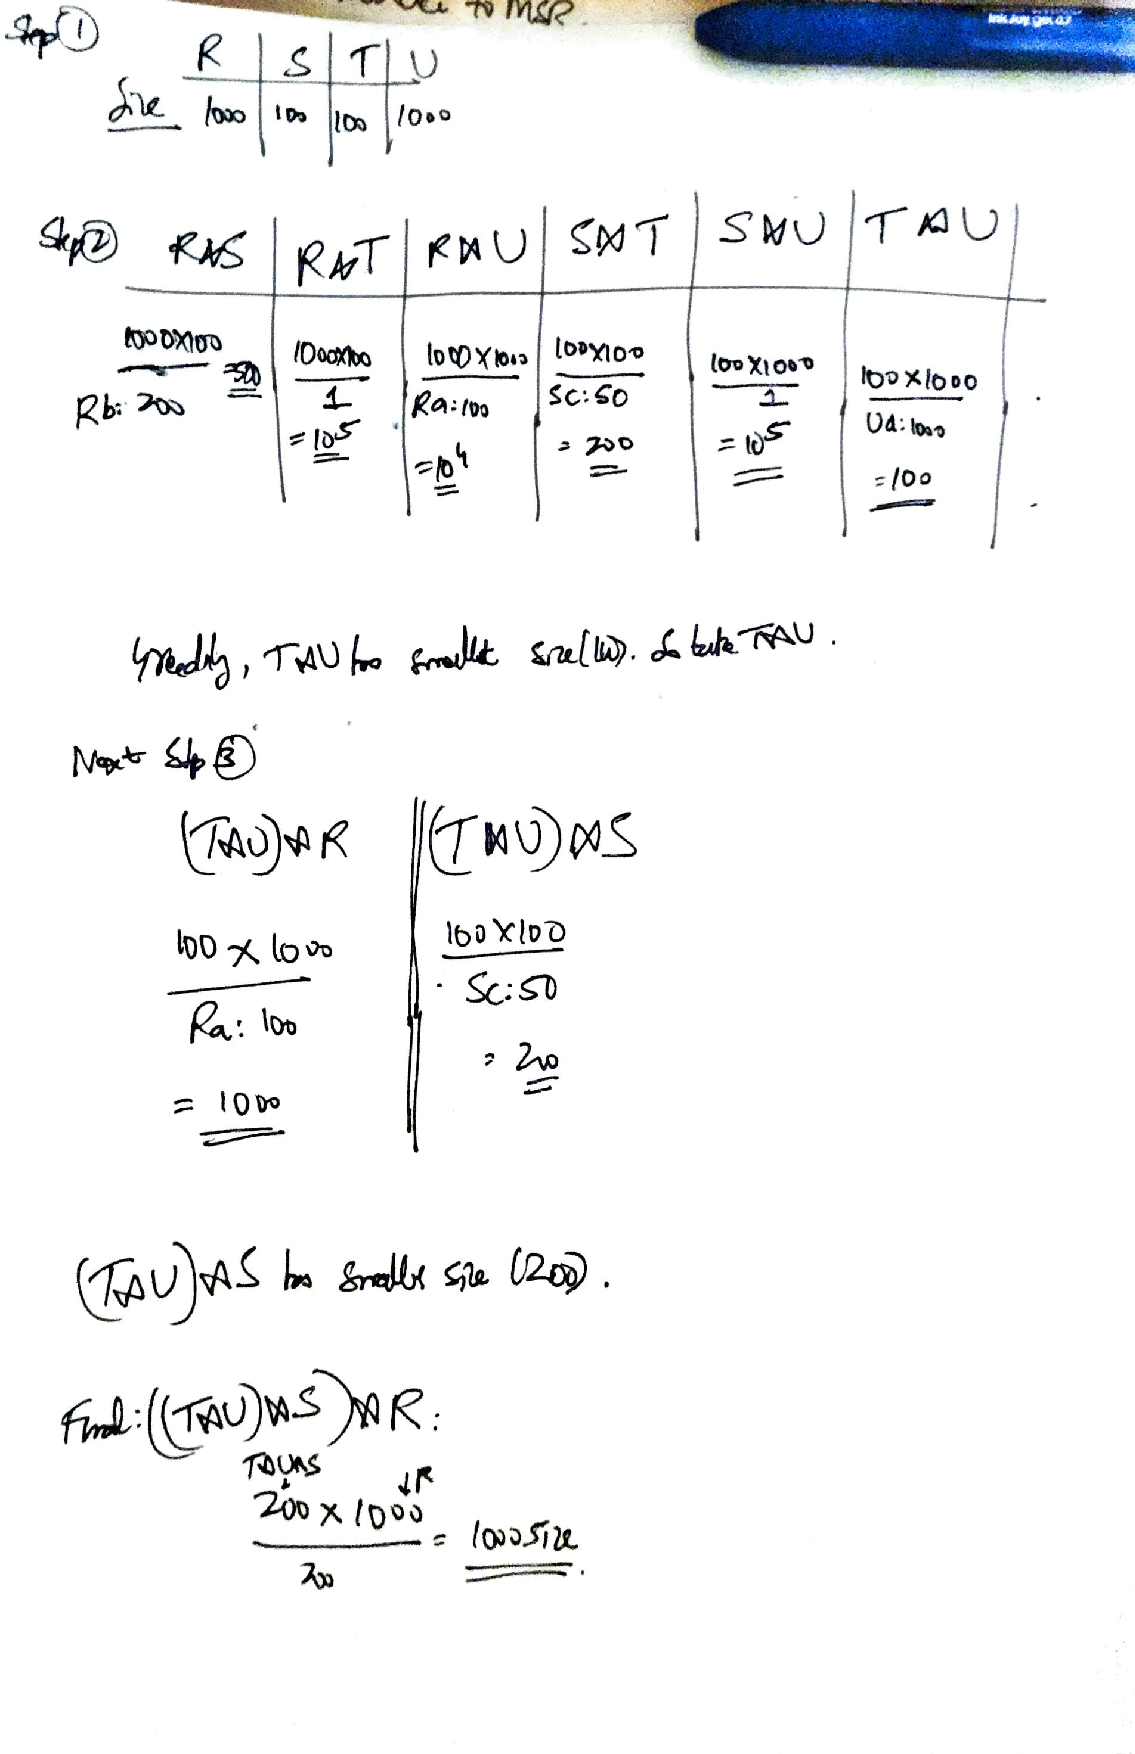
\includegraphics[width=\textwidth]{db-q4-1.pdf}

\subsubsection{Cost calculation:}
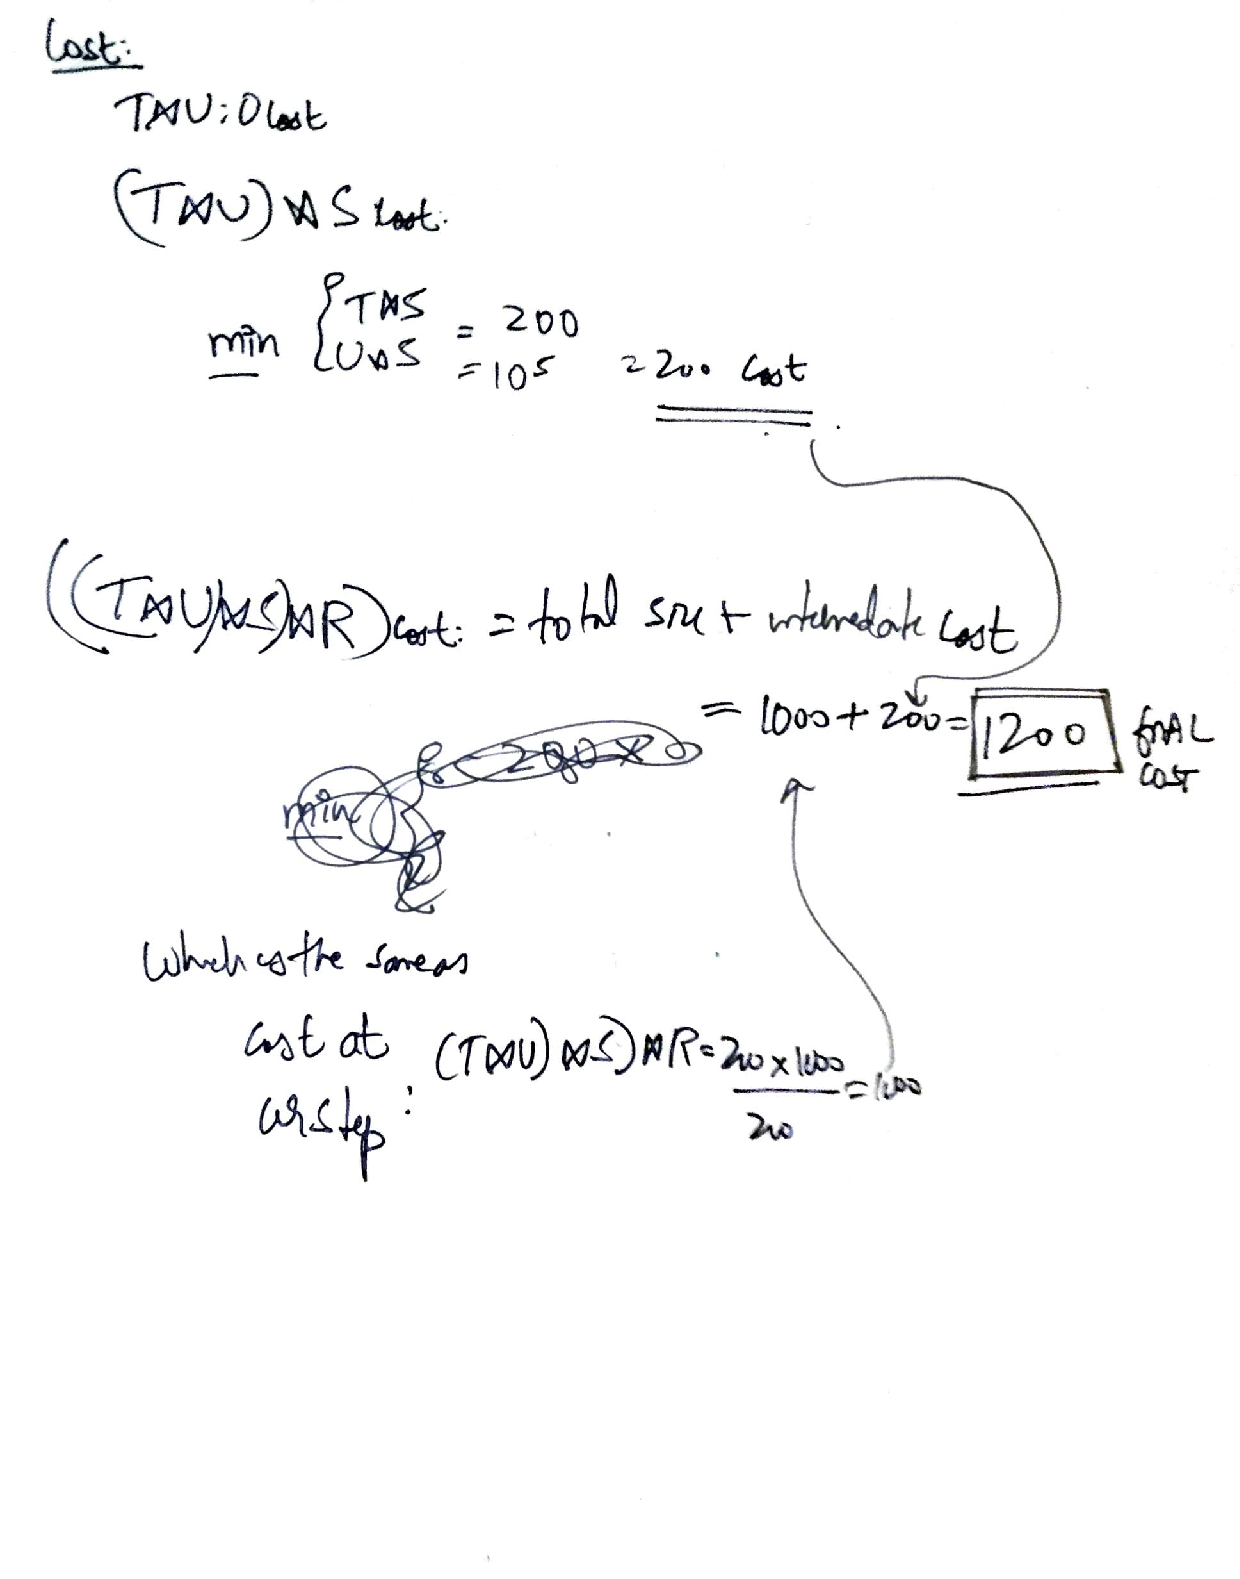
\includegraphics[width=\textwidth]{db-q4-2.pdf}
\section{Q5}

\subsubsection{Q5.1}
After \texttt{<U, B, 20>}, we have transactions $T$ and $U$ active.  So, to start the checkpoint,
we have to write \texttt{<START CKPT(T, U)>}. 

Transaction $T$ is committed after transaction $U$. So to end, we have  to
write \texttt{<END CKPT>} record after \texttt{<COMMIT T>}.

\subsubsection{Q5.2}

For \texttt{<V, B, 80>}, we only need to undo \texttt{<V, B, 80>} since
we have a \texttt{<END CKPT>} checkpoint right before it. 

For \texttt{<U, D, 40>}, we must look back till \texttt{START T} since that
is the earliest transaction that we active during the checkpoint.


For \texttt{<T, A, 10>}, we must look back till the \emph{previous}
checkpoint --- not the one being discussed in the question, since it
occured even before the current checkpoint started recoding.

\section{Q6}

When we insert $0011$, there are four records for bucket 0, which overflows.
Adding a second bit to the bucket addresses doesn't help, because the first
four records all begin with $00$. Thus, we go to $i = 3$ and use the first three
bits for each bucket address. Now we have space for $4$ records in each bucket;
however, we can get at maximum $2$ records per bucket --- we have 4 bit hashes,
our buckets are keyed by 3 bits, leaving 1 bit of ambiguity. 1 bit 
can be 2 records. When $1111$ is inserted, we have two records in each bucket.

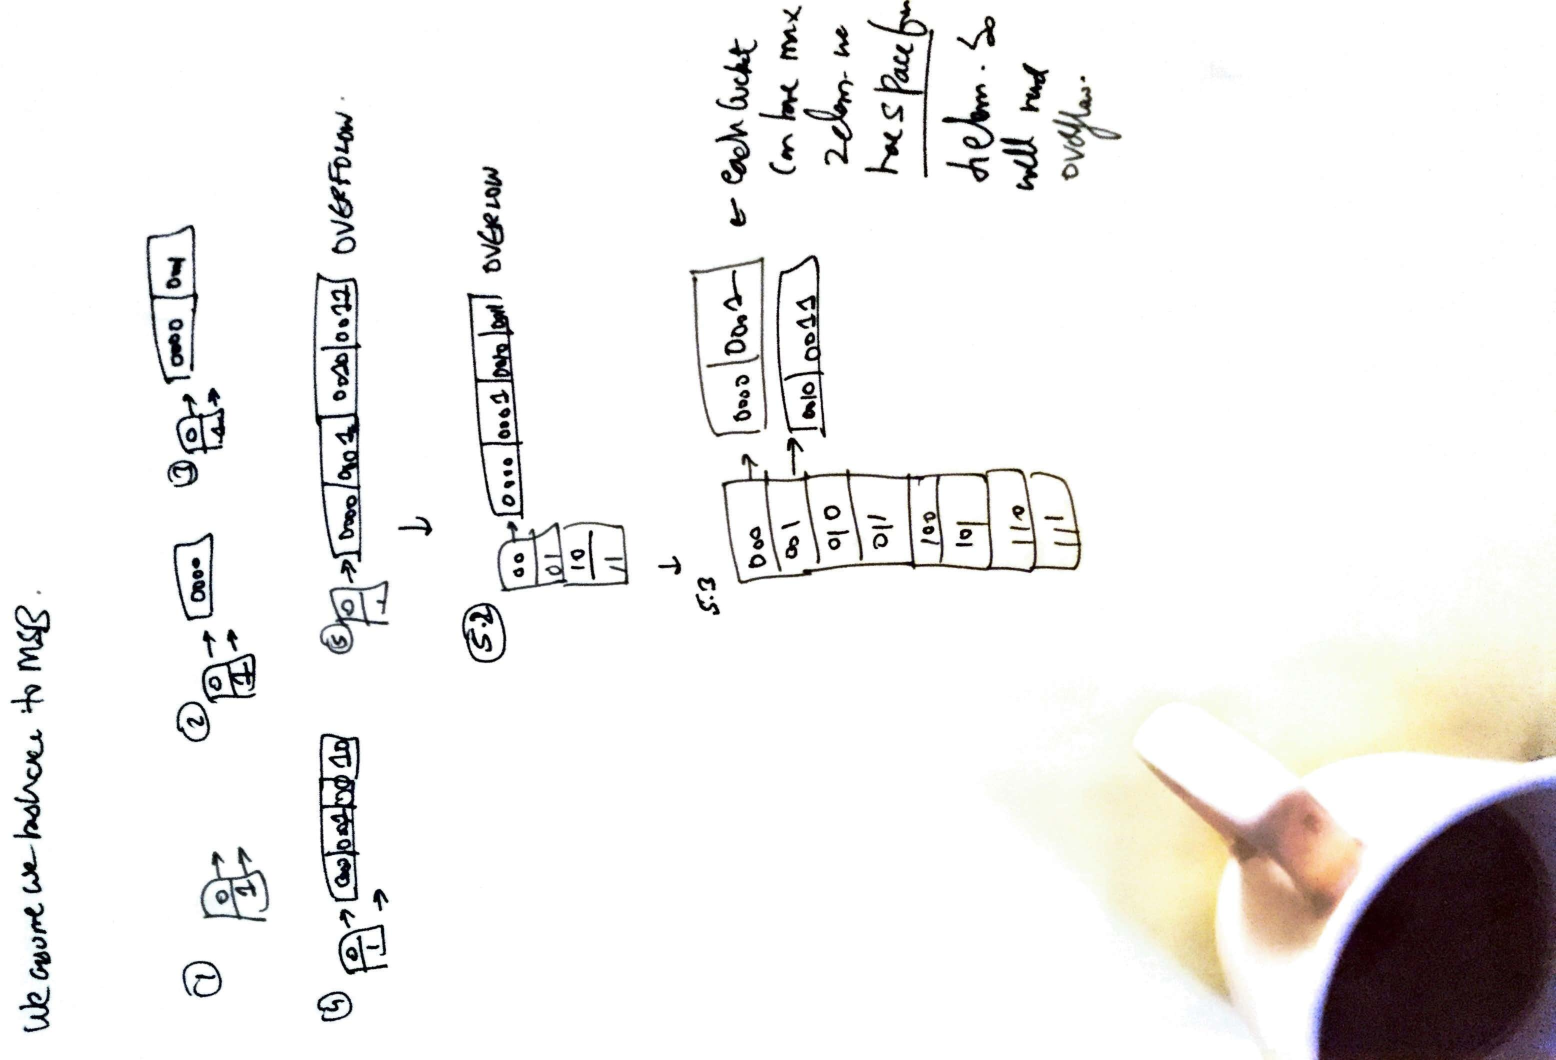
\includegraphics[width=\textwidth, angle=270]{db-q6.pdf}

\section{Q7}
\subsubsection{Q7.1}
$SL_x(E)$ for a shared lock by transaction $x$ on elem $E$. $U_x(E)$ for
unlock by transaction $x$ on elem $E$.

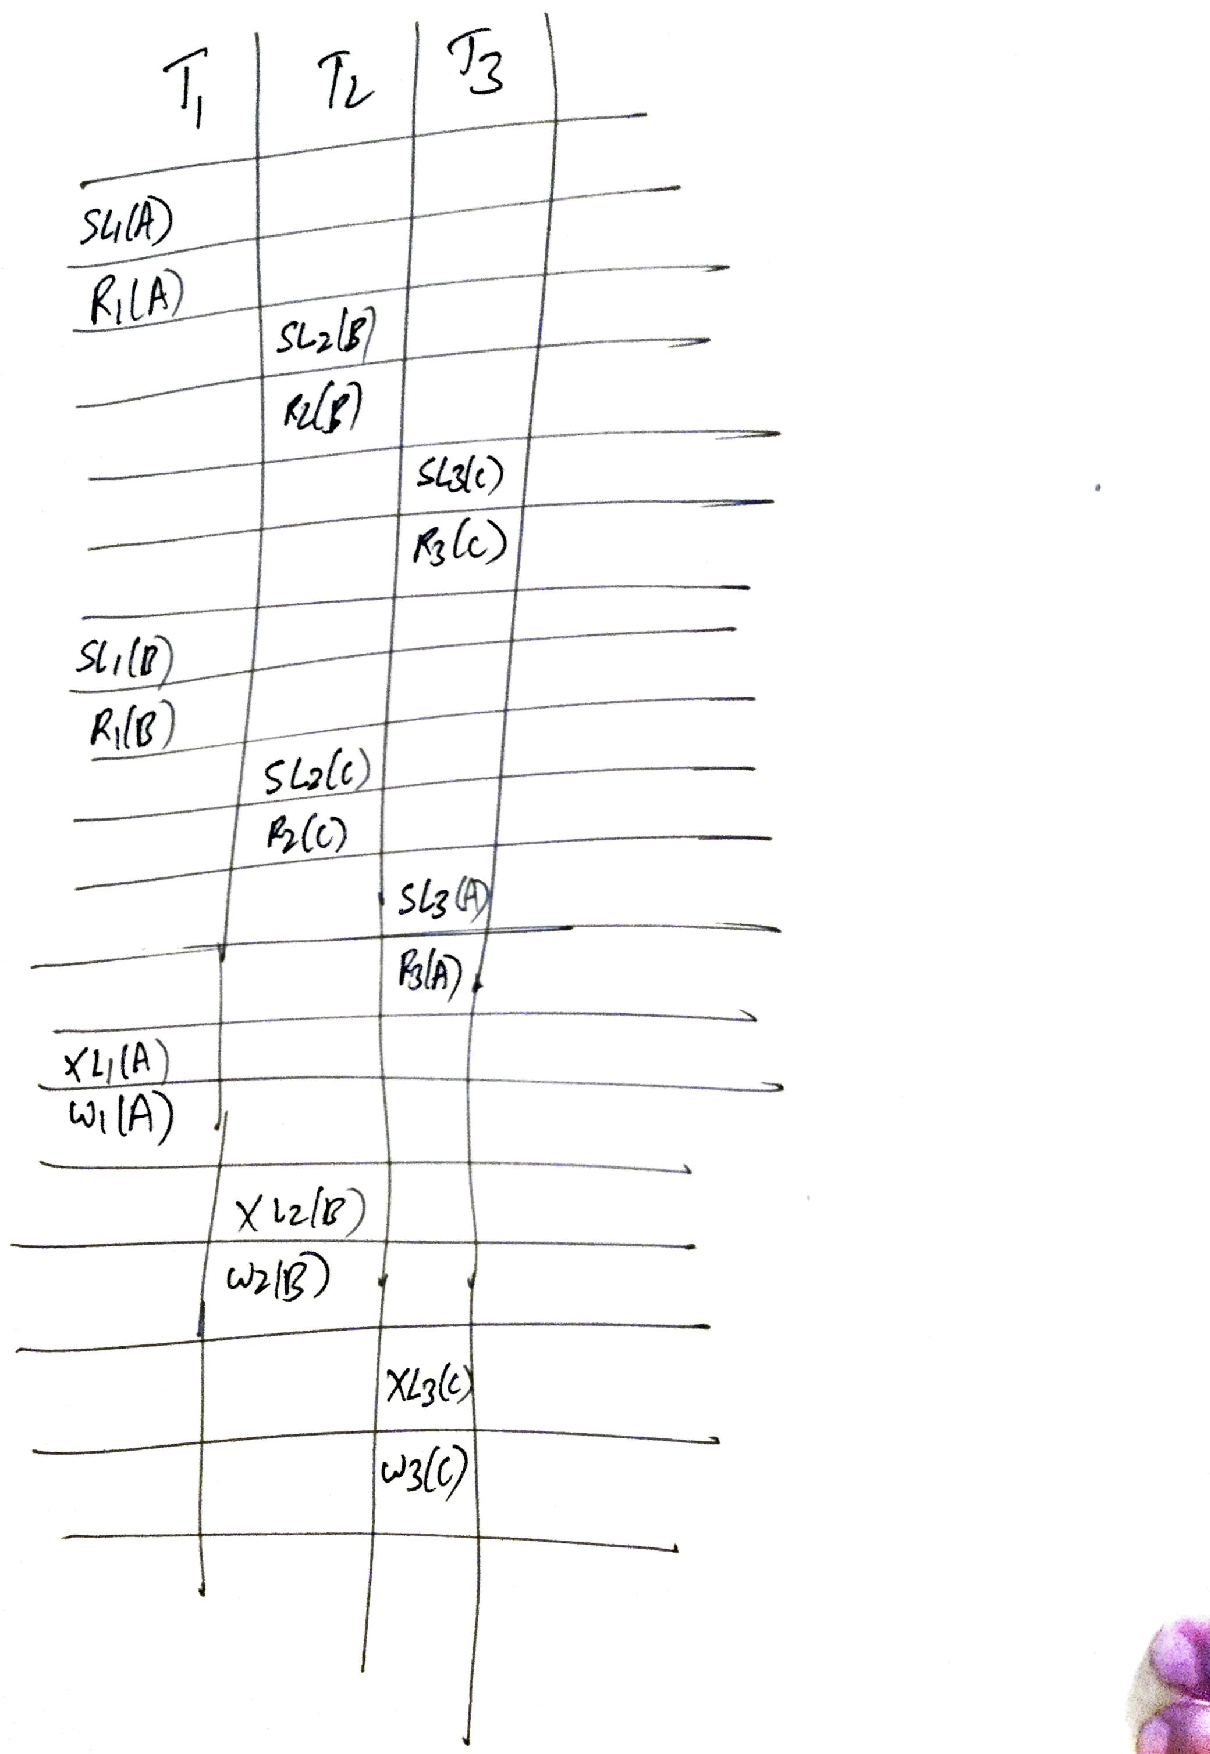
\includegraphics[width=0.8\textwidth]{db-q71.pdf}

All locks are accepted, since there are no conflicting locks.

\subsubsection{Q7.2}

Table will be the same as for the above, since we did not have any read action
which was followed by a write action of the same element by the same
transaction.


\subsubsection{Q7.3}


\section{Q8}
\begin{align*}
    &r_1(O_1) \mapsto \text{$T_1$ puts }IS(B_1); S(O_1); \texttt{release} \\
    &r_2(O_2) \mapsto \text{$T_2$ puts }IS(B_1); S(O_2); \texttt{release}\\
    &r_3(O_1) \mapsto \text{$T_3$ puts }IS(B_2); S(O_3); \texttt{release}\\
    &w_1(O_3) \mapsto \text{$T_1$ puts }IX(B_2); X(O_3); \texttt{release}\\
    &w_2(O_4) \mapsto \text{$T_2$ puts }IX(B_2); X(O_4); \texttt{release}\\
    &w_3(O_5) \mapsto \text{$T_3$ puts }IX(B_2); X(O_5); \texttt{release}\\
    &w_1(O_2) \mapsto \text{$T_1$ puts }IX(B_2); X(O_3); \texttt{release}\\
\end{align*}
\section{Q9}
\subsubsection{9.1}
In Undo Logging Logging, we need to write all we need to write all modified
data to disk before committing a transaction.  This may need a large number of disk
I/O’s. This is unlike the case of Redo logging, which allows changes to be
present in-memory; only need to flush changes before committing.

\subsubsection{9.2}
Selinger optimization improves upon DP approach by keeping for
each  not only the plan of least cost, but also plans that have higher
cost but produce a result that is sorted in an order that may
be useful for parent queries.
\subsubsection{9.3}

View serializable: If a given schedule is found to be view equivalent to some serial schedule. Alternatively,
  there are no cycles in the dependency graph.
Conflict serializable: If there are no cycles in the conflict graph.


Intuitively, view-serializability considers all the connections between
transactions T and U such that T writes a database element whose value U
reads. 

The key difference between view, conflict serializability happens
when a transaction T writes a value A that no other transaction reads (since
all other transactions later write their own values for A). In this case, the
$WT(A)$ action can be placed in certain other positions of the schedule (where A
is likewise never read) that would not be permitted under the definition of
conflict-serializability. Hence, view serializability is more flexible
than conflict serializability.

Therefore, every conflict serializable schedule is indeed view serializable.
But there can be some freedom used by the view serializable version that
the conflict serializable version cannot use.


\subsubsection{9.4}

We can use strict 2-phase locking for recoverability. This requires that
in addition to the lock being 2-Phase, all Exclusive(X) Locks held by the
transaction be released until after the Transaction Commits.

\subsubsection{9.5}
Database operations are in fact relational algebra operations. These
operations are pure mathematical expressions, and are generally reads or
writes into disjoint pieces of data. This makes them naturally parallelizable.

Many DB operations such as projections work tuple-at-a-time, which can be
parallelized across tuples. If we have the hashes of relations, we can
compute union, intersection, and difference all in parallel.


\subsubsection{9.6}
File system does not generally have multiple readers and writers to a single
file. It also does not need to manage structured data. Hence, many of the ACID
like concerns simply do not occur in the case of a file system.

\subsubsection{9.7}
the commit bit for X is true if and only if the most recent
transaction to write X has already committed. The purpose of this bit
is to avoid a situation where one transaction T reads data written by
another transaction U, and U then aborts. This problem, where T makes
a "dirty read" of uncommitted data, certainly can cause the database
state to become inconsistent, and any scheduler needs a mechanism to
prevent dirty reads.

\subsubsection{9.8}
\begin{itemize}
        \item  Two-phase locking - 2PL.
        \item General lock based solutions.
        \item Timestamp ordering.
        \item Validation based concurrency control.
\end{itemize}

Increment based locking is good in this case because it allows to add or subtract a constant
from an element, which is what most kinds of bank transaactions are. Increment locks on the same
element do not conflict with each other.
\subsubsection{9.9}

The first task of the recovery manager is to divide the transactions into
committed and uncommitted transactions. If there is a log record <COMMIT T>,
then by undo rule f/2 all changes made by transaction T were previously written
to disk. Thus, T by itself could not have left the database in an inconsistent
state when the system failure occurred.
However, suppose that we find a <START T> record on the log but no
<COMMIT T> record. Then there could have been some changes to the database
made by T that got written to disk before the crash, while other changes by
T either were not made, even in the main-memory buffers, or were made in
the buffers but not copied to disk. In this case, T is an incomplete transaction
and must be undone.

\subsubsection{9.10}
all trees of n vertices is $n^{n-2}$. Number of left-deep trees is $n!$.
$n^{n-2}$ is much larger than $n!$.


\end{document}
